% answers.tex —— 1988 年·全国卷·文科 · 参考答案与详细解析片段
% 由 tools/generate_projects.py 依来源总账自 1988/1988_数学真题_全国文_试题.md + 1988/1988_数学真题_全国文_解析正文.md + 1988/1988_数学真题_全国文_答案要点.md 生成，勿手改（改源 MD 后重跑）


\begin{gktip}
固定源只有一页题面，没有答案和解析页。以下各题结论均为本库独立复算；第 4、12、22 题的图形依据固定源重绘。
\end{gktip}

\begin{answer}
\gksolhead{1}{}

\textbf{题目}：

\Needspace{5\baselineskip}
复数

\nopagebreak[4]
\[
\left(\frac{1-i}{1+i}\right)^2
\]

的值等于\mbox{（　　）}

（A）$1$　　（B）$-1$　　（C）$i$　　（D）$-i$

\Needspace{4\baselineskip}
\textbf{解析}

\Needspace{5\baselineskip}
有

\nopagebreak[4]
\[
\frac{1-i}{1+i}=-i,
\]

所以原式为 $(-i)^2=-1$，答案为 B。

\gkanswer{答案：B}

\end{answer}
\begin{answer}
\gksolhead{2}{}

\textbf{题目}：

\Needspace{5\baselineskip}
圆 $M$ 的方程为

\nopagebreak[4]
\[
(x-3)^2+(y-2)^2=2,
\]

\Needspace{5\baselineskip}
直线 $L$ 的方程为

\nopagebreak[4]
\[
x+y-3=0,
\]

点 $P$ 的坐标为 $(2,1)$，那么\mbox{（　　）}

（A）点 $P$ 在直线 $L$ 上，但不在圆 $M$ 上

（B）点 $P$ 在圆 $M$ 上，但不在直线 $L$ 上

（C）点 $P$ 既在圆 $M$ 上，又在直线 $L$ 上

（D）点 $P$ 既不在直线 $L$ 上，也不在圆 $M$ 上

\Needspace{4\baselineskip}
\textbf{解析}

\Needspace{5\baselineskip}
点 $P=(2,1)$ 满足 $x+y-3=0$，且

\nopagebreak[4]
\[
(2-3)^2+(1-2)^2=2.
\]

所以点 $P$ 同时在圆 $M$ 和直线 $L$ 上，答案为 C。

\gkanswer{答案：C}

\end{answer}
\begin{answer}
\gksolhead{3}{}

\textbf{题目}：

集合 $\{1,2,3\}$ 的子集共有\mbox{（　　）}

（A）5 个　　（B）6 个　　（C）7 个　　（D）8 个

\Needspace{4\baselineskip}
\textbf{解析}

\Needspace{5\baselineskip}
三个元素的集合共有

\nopagebreak[4]
\[
2^3=8
\]

个子集，答案为 D。

\gkanswer{答案：D}

\end{answer}
\begin{answer}
\gksolhead{4}{}

\textbf{题目}：

\Needspace{5\baselineskip}
函数

\nopagebreak[4]
\[
y=a^x\qquad(0<a<1)
\]

的图象是\mbox{（　　）}
\nopagebreak[4]
\begin{center}% 1988 年全国卷文科第 4 题：指数函数图象的四个选项
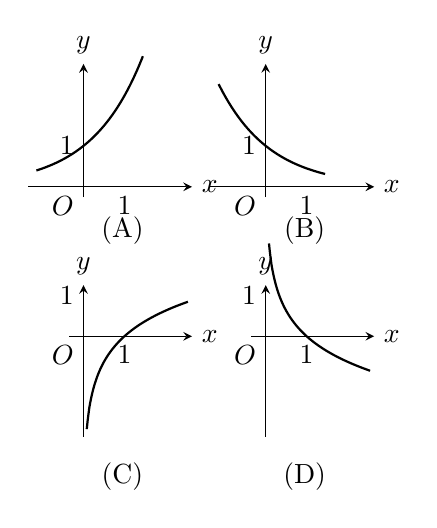
\begin{tikzpicture}[scale=0.52,>=stealth]
  \begin{scope}
    \draw[->] (-1.35,0)--(2.65,0) node[right] {$x$};
    \draw[->] (0,-0.25)--(0,3.0) node[above] {$y$};
    \draw[thick,domain=-1.15:1.45,samples=100]
      plot (\x,{exp(0.8*\x)});
    \node[left] at (0,1) {$1$};
    \node[below] at (1,0) {$1$};
    \node[below left] at (0,0) {$O$};
    \node[below] at (0.95,-0.5) {(A)};
  \end{scope}

  \begin{scope}[xshift=4.45cm]
    \draw[->] (-1.35,0)--(2.65,0) node[right] {$x$};
    \draw[->] (0,-0.25)--(0,3.0) node[above] {$y$};
    \draw[thick,domain=-1.15:1.45,samples=100]
      plot (\x,{exp(-0.8*\x)});
    \node[left] at (0,1) {$1$};
    \node[below] at (1,0) {$1$};
    \node[below left] at (0,0) {$O$};
    \node[below] at (0.95,-0.5) {(B)};
  \end{scope}

  \begin{scope}[yshift=-3.65cm]
    \draw[->] (-0.35,0)--(2.65,0) node[right] {$x$};
    \draw[->] (0,-2.45)--(0,1.25) node[above] {$y$};
    \draw[thick,domain=0.08:2.55,samples=120]
      plot (\x,{0.9*ln(\x)});
    \node[left] at (0,1) {$1$};
    \node[below] at (1,0) {$1$};
    \node[below left] at (0,0) {$O$};
    \node[below] at (0.95,-2.85) {(C)};
  \end{scope}

  \begin{scope}[xshift=4.45cm,yshift=-3.65cm]
    \draw[->] (-0.35,0)--(2.65,0) node[right] {$x$};
    \draw[->] (0,-2.45)--(0,1.25) node[above] {$y$};
    \draw[thick,domain=0.08:2.55,samples=120]
      plot (\x,{-0.9*ln(\x)});
    \node[left] at (0,1) {$1$};
    \node[below] at (1,0) {$1$};
    \node[below left] at (0,0) {$O$};
    \node[below] at (0.95,-2.85) {(D)};
  \end{scope}
\end{tikzpicture}
\end{center}
\nopagebreak[4]
\Needspace{4\baselineskip}
\textbf{解析}

当 $0<a<1$ 时，指数函数 $y=a^x$ 随 $x$ 增大而减小，并且恒为正、经过 $(0,1)$，对应图形 B。

\gkanswer{答案：B}

\end{answer}
\begin{answer}
\gksolhead{5}{}

\textbf{题目}：

\Needspace{5\baselineskip}
已知椭圆方程

\nopagebreak[4]
\[
\frac{x^2}{20}+\frac{y^2}{11}=1,
\]

那么它的焦距是\mbox{（　　）}

（A）$6$　　（B）$3$　　（C）$2\sqrt{31}$　　（D）$\sqrt{31}$

\Needspace{4\baselineskip}
\textbf{解析}

\Needspace{5\baselineskip}
椭圆参数满足

\nopagebreak[4]
\[
c^2=a^2-b^2=20-11=9,
\qquad c=3.
\]

焦距为 $2c=6$，答案为 A。

\gkanswer{答案：A}

\end{answer}
\begin{answer}
\gksolhead{6}{}

\textbf{题目}：

\Needspace{5\baselineskip}
在复平面内，与复数

\nopagebreak[4]
\[
z=-1-i
\]

的共轭复数对应的点位于\mbox{（　　）}

（A）第一象限　　（B）第二象限　　（C）第三象限　　（D）第四象限

\Needspace{4\baselineskip}
\textbf{解析}

\Needspace{5\baselineskip}
复数 $z=-1-i$ 的共轭复数为

\nopagebreak[4]
\[
\overline z=-1+i,
\]

实部为负、虚部为正，故对应点在第二象限，答案为 B。

\gkanswer{答案：B}

\end{answer}
\begin{answer}
\gksolhead{7}{}

\textbf{题目}：

\Needspace{5\baselineskip}
在

\nopagebreak[4]
\[
(x-\sqrt3)^{10}
\]

的展开式中，$x^6$ 的系数是\mbox{（　　）}

（A）$-27C_{10}^{6}$　　（B）$27C_{10}^{4}$

（C）$-9C_{10}^{6}$　　（D）$9C_{10}^{4}$

\Needspace{4\baselineskip}
\textbf{解析}

\Needspace{5\baselineskip}
要得到 $x^6$ 项，选择四个 $-\sqrt3$ 因子和六个 $x$ 因子，系数为

\nopagebreak[4]
\[
\binom{10}{4}(-\sqrt3)^4
=9\binom{10}{4}.
\]

答案为 D。

\gkanswer{答案：D}

\end{answer}
\begin{answer}
\gksolhead{8}{}

\textbf{题目}：

\Needspace{5\baselineskip}
函数

\nopagebreak[4]
\[
y=3\cos\left(\frac25x-\frac\pi6\right)
\]

的最小正周期是\mbox{（　　）}

（A）$\frac25\pi$　　（B）$\frac52\pi$　　（C）$2\pi$　　（D）$5\pi$

\Needspace{4\baselineskip}
\textbf{解析}

\Needspace{5\baselineskip}
余弦函数的角频率为 $2/5$，故最小正周期

\nopagebreak[4]
\[
T=\frac{2\pi}{2/5}=5\pi.
\]

答案为 D。

\gkanswer{答案：D}

\end{answer}
\begin{answer}
\gksolhead{9}{}

\textbf{题目}：

$\sin\left(-\dfrac{19}{6}\pi\right)$ 的值等于\mbox{（　　）}

（A）$\frac12$　　（B）$-\frac12$　　（C）$\frac{\sqrt3}{2}$　　（D）$-\frac{\sqrt3}{2}$

\Needspace{4\baselineskip}
\textbf{解析}

\nopagebreak[4]
\[
-\frac{19\pi}{6}+4\pi=\frac{5\pi}{6},
\]

\Needspace{5\baselineskip}
所以

\nopagebreak[4]
\[
\sin\left(-\frac{19\pi}{6}\right)=\sin\frac{5\pi}{6}=\frac12.
\]

答案为 A。

\gkanswer{答案：A}

\end{answer}
\begin{answer}
\gksolhead{10}{}

\textbf{题目}：

\Needspace{5\baselineskip}
直线

\nopagebreak[4]
\[
x+ay=2a+2
\]

\Needspace{5\baselineskip}
与直线

\nopagebreak[4]
\[
ax+y=a+1
\]

平行（不重合）的充要条件是\mbox{（　　）}

（A）$a=\frac12$　　（B）$a=-\frac12$　　（C）$a=1$　　（D）$a=-1$

\Needspace{4\baselineskip}
\textbf{解析}

\Needspace{5\baselineskip}
两直线平行要求法向量 $(1,a)$ 与 $(a,1)$ 平行，即

\nopagebreak[4]
\[
a^2=1.
\]

当 $a=-1$ 时两方程分别化为 $x-y=0$ 与 $x-y=0$，重合；当 $a=1$ 时为两条不同的平行线。因此答案为 C。

\gkanswer{答案：C}

\end{answer}
\begin{answer}
\gksolhead{11}{}

\textbf{题目}：

\Needspace{5\baselineskip}
函数

\nopagebreak[4]
\[
y=\frac{x-2}{2x-1}\qquad\left(x\in R,\ x\ne\frac12\right)
\]

的反函数是\mbox{（　　）}

（A）$y=\frac{x-2}{2x-1}\ (x\in R,\ x\ne\frac12)$

（B）$y=\frac{2x-1}{x-2}\ (x\in R,\ x\ne2)$

（C）$y=\frac{x+2}{2x-1}\ (x\in R,\ x\ne\frac12)$

（D）$y=\frac{2x-1}{x+2}\ (x\in R,\ x\ne-2)$

\Needspace{4\baselineskip}
\textbf{解析}

\Needspace{5\baselineskip}
设反函数自变量为 $y$，由

\nopagebreak[4]
\[
y=\frac{x-2}{2x-1}
\]

\Needspace{5\baselineskip}
解得

\nopagebreak[4]
\[
x=\frac{y-2}{2y-1}.
\]

\Needspace{5\baselineskip}
交换变量后反函数仍为

\nopagebreak[4]
\[
y=\frac{x-2}{2x-1},\qquad x\ne\frac12,
\]

答案为 A。

\gkanswer{答案：A}

\end{answer}
\begin{answer}
\gksolhead{12}{}

\textbf{题目}：

如图，正四棱台中，$A'D'$ 所在的直线与 $BB'$ 所在的直线是\mbox{（　　）}
\nopagebreak[4]
\begin{center}% 1988 年全国卷文科第 12 题：正四棱台
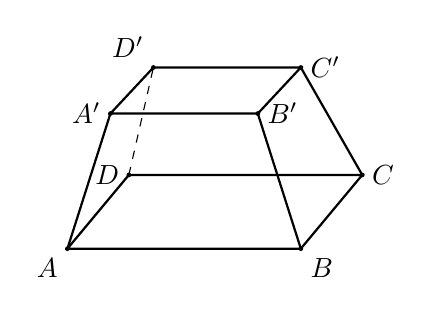
\begin{tikzpicture}[scale=0.78,>=stealth]
  \coordinate (A) at (0,0);
  \coordinate (B) at (3.8,0);
  \coordinate (C) at (4.8,1.2);
  \coordinate (D) at (1.0,1.2);
  \coordinate (Ap) at (0.7,2.2);
  \coordinate (Bp) at (3.1,2.2);
  \coordinate (Cp) at (3.8,2.95);
  \coordinate (Dp) at (1.4,2.95);
  \draw[thick] (A)--(B)--(C)--(D)--cycle;
  \draw[thick] (Ap)--(Bp)--(Cp)--(Dp)--cycle;
  \draw[thick] (A)--(Ap) (B)--(Bp) (C)--(Cp);
  \draw[dashed] (D)--(Dp);
  \fill (A) circle (1.1pt) node[below left] {$A$};
  \fill (B) circle (1.1pt) node[below right] {$B$};
  \fill (C) circle (1.1pt) node[right] {$C$};
  \fill (D) circle (1.1pt) node[left] {$D$};
  \fill (Ap) circle (1.1pt) node[left] {$A'$};
  \fill (Bp) circle (1.1pt) node[right] {$B'$};
  \fill (Cp) circle (1.1pt) node[right] {$C'$};
  \fill (Dp) circle (1.1pt) node[above left] {$D'$};
\end{tikzpicture}
\end{center}
\nopagebreak[4]
（A）相交直线　　（B）平行直线

（C）不互相垂直的异面直线　　（D）互相垂直的异面直线

\Needspace{4\baselineskip}
\textbf{解析}

在正四棱台中，$A'D'$ 平行于底面边 $AD$，而 $BB'$ 是侧棱。两线既不相交也不平行；由正四棱台的空间位置，侧棱方向与 $A'D'$ 不垂直。因此它们是不互相垂直的异面直线，答案为 C。

\gkanswer{答案：C}

\end{answer}
\begin{answer}
\gksolhead{13}{}

\textbf{题目}：

\Needspace{5\baselineskip}
函数

\nopagebreak[4]
\[
y=\sin\left(x+\frac\pi4\right)
\]

在闭区间\mbox{（　　）}上是增函数

（A）$\left[-\frac\pi2,\frac\pi2\right]$　　（B）$\left[-\frac{3\pi}{4},\frac\pi4\right]$

（C）$[-\pi,0]$　　（D）$\left[-\frac\pi4,\frac{3\pi}{4}\right]$

\Needspace{4\baselineskip}
\textbf{解析}

\Needspace{5\baselineskip}
正弦函数在自变量区间

\nopagebreak[4]
\[
\left[-\frac\pi2,\frac\pi2\right]
\]

\Needspace{5\baselineskip}
上递增，所以令 $x+\pi/4$ 落在该区间，得到

\nopagebreak[4]
\[
x\in\left[-\frac{3\pi}{4},\frac\pi4\right].
\]

答案为 B。

\gkanswer{答案：B}

\end{answer}
\begin{answer}
\gksolhead{14}{}

\textbf{题目}：

假设在 200 件产品中有 3 件次品，现在从中任意抽取 5 件，其中至少有 2 件次品的抽法有\mbox{（　　）}

（A）$C_3^2C_{197}^3+C_3^3C_{197}^2$ 种

（B）$C_3^2C_{197}^3$ 种

（C）$C_{200}^5-C_{197}^5$ 种

（D）$C_{200}^5-C_3^1C_{197}^4$ 种

\Needspace{4\baselineskip}
\textbf{解析}

\Needspace{5\baselineskip}
至少抽到两件次品有两种互斥情形：

\nopagebreak[4]
\[
C_3^2C_{197}^3+C_3^3C_{197}^2.
\]

答案为 A。

\gkanswer{答案：A}

\end{answer}
\begin{answer}
\gksolhead{15}{}

\textbf{题目}：

已知二面角 $\alpha-AB-\beta$ 的平面角是锐角 $\theta$，$\alpha$ 内一点 $C$ 到 $\beta$ 的距离为 $3$，点 $C$ 到棱 $AB$ 的距离为 $4$，那么 $\tan\theta$ 的值等于\mbox{（　　）}

（A）$\frac34$　　（B）$\frac35$　　（C）$\frac{3\sqrt7}{7}$　　（D）$\frac{\sqrt7}{3}$

\Needspace{4\baselineskip}
\textbf{解析}

\Needspace{5\baselineskip}
在垂直于棱 $AB$ 的截面内，二面角的平面角为 $\theta$。点 $C$ 到平面 $\beta$ 的距离等于点 $C$ 到棱的距离乘以 $\sin\theta$，所以

\nopagebreak[4]
\[
3=4\sin\theta.
\]

\Needspace{5\baselineskip}
因 $\theta$ 为锐角，

\nopagebreak[4]
\[
\tan\theta=\frac{3}{\sqrt{16-9}}=\frac3{\sqrt7}
=\frac{3\sqrt7}{7}.
\]

答案为 C。

\gkanswer{答案：C}

\end{answer}
\begin{answer}
\gksolhead{16}{}

\textbf{题目}：

\Needspace{5\baselineskip}
求复数

\nopagebreak[4]
\[
\sqrt3-i
\]

的模和辐角的主值。

\Needspace{4\baselineskip}
\textbf{解析}

\nopagebreak[4]
\[
|\sqrt3-i|=2,
\]

且复数位于第四象限，故辐角主值为 $-\pi/6$。

\gkanswer{答案：模为 $2$，辐角主值为 $-\dfrac\pi6$}

\end{answer}
\begin{answer}
\gksolhead{17}{}

\textbf{题目}：

\Needspace{5\baselineskip}
解方程

\nopagebreak[4]
\[
9^{-x}-2\cdot3^{1-x}=27.
\]

\Needspace{4\baselineskip}
\textbf{解析}

\Needspace{5\baselineskip}
令 $u=3^{-x}>0$，则方程化为

\nopagebreak[4]
\[
u^2-6u-27=0
= (u-9)(u+3)=0.
\]

取正根 $u=9$，得到 $x=-2$。

\gkanswer{答案：$x=-2$}

\end{answer}
\begin{answer}
\gksolhead{18}{}

\textbf{题目}：

\Needspace{5\baselineskip}
已知

\nopagebreak[4]
\[
\sin\theta=-\frac35,\qquad
3\pi<\theta<\frac{7\pi}{2},
\]

\Needspace{5\baselineskip}
求

\nopagebreak[4]
\[
\tan\frac\theta2.
\]

\Needspace{4\baselineskip}
\textbf{解析}

\Needspace{5\baselineskip}
区间 $3\pi<\theta<7\pi/2$ 的终边位于第三象限，所以

\nopagebreak[4]
\[
\cos\theta=-\frac45.
\]

\Needspace{5\baselineskip}
因此

\nopagebreak[4]
\[
\tan\frac\theta2
=\frac{\sin\theta}{1+\cos\theta}
=\frac{-3/5}{1/5}=-3.
\]

\gkanswer{答案：$\tan\dfrac\theta2=-3$}

\end{answer}
\begin{answer}
\gksolhead{19}{}

\textbf{题目}：

一个直角三角形的两条直角边的长分别为 $3\text{ cm}$ 和 $4\text{ cm}$，将这个直角三角形以斜边为轴旋转一周，求所得旋转体的体积。

\Needspace{4\baselineskip}
\textbf{解析}

\Needspace{5\baselineskip}
将直角三角形以斜边为轴旋转，所得立体是两个共底圆锥的组合。设斜边为 $5$，三角形面积为 $6$，对斜边的高为

\nopagebreak[4]
\[
h=\frac{2\cdot3\cdot4}{5}=\frac{12}{5}.
\]

\Needspace{5\baselineskip}
三角形重心到斜边的距离为 $h/3=4/5$。由帕普斯定理，旋转体体积为

\nopagebreak[4]
\[
V=6\cdot2\pi\cdot\frac45
=\frac{48\pi}{5}\text{ cm}^3.
\]

\gkanswer{答案：$\dfrac{48\pi}{5}\text{ cm}^3$}

\end{answer}
\begin{answer}
\gksolhead{20}{}

\textbf{题目}：

\Needspace{5\baselineskip}
求极限

\nopagebreak[4]
\[
\lim_{n\to\infty}\frac{3n^2+2n}{n^2+3n-1}.
\]

\Needspace{4\baselineskip}
\textbf{解析}

\Needspace{5\baselineskip}
分子分母同除以 $n^2$：

\nopagebreak[4]
\[
\lim_{n\to\infty}\frac{3+2/n}{1+3/n-1/n^2}=3.
\]

\gkanswer{答案：$3$}

\end{answer}
\begin{answer}
\gksolhead{21}{}

\textbf{题目}：

\Needspace{5\baselineskip}
证明：

\nopagebreak[4]
\[
\cos3\alpha=4\cos^3\alpha-3\cos\alpha.
\]

\Needspace{4\baselineskip}
\textbf{解析}

\Needspace{5\baselineskip}
由和角公式

\nopagebreak[4]
\[
\cos3\alpha=\cos(2\alpha+\alpha)
=\cos2\alpha\cos\alpha-\sin2\alpha\sin\alpha.
\]

\Needspace{5\baselineskip}
代入 $\cos2\alpha=2\cos^2\alpha-1$、$\sin2\alpha=2\sin\alpha\cos\alpha$，得

\nopagebreak[4]
\[
\cos3\alpha
=(2\cos^2\alpha-1)\cos\alpha
-2\sin^2\alpha\cos\alpha
=4\cos^3\alpha-3\cos\alpha.
\]

\gkanswer{答案：恒等式成立。}

\end{answer}
\begin{answer}
\gksolhead{22}{}

\textbf{题目}：

\Needspace{5\baselineskip}
如图，四棱锥 $S-ABCD$ 的底面是边长为 $1$ 的正方形，侧棱 $SB$ 垂直于底面，并且

\nopagebreak[4]
\[
SB=\sqrt3.
\]

用 $\alpha$ 表示 $\angle ASD$，求 $\sin\alpha$。
\nopagebreak[4]
\begin{center}% 1988 年全国卷文科第 22 题：四棱锥 S-ABCD
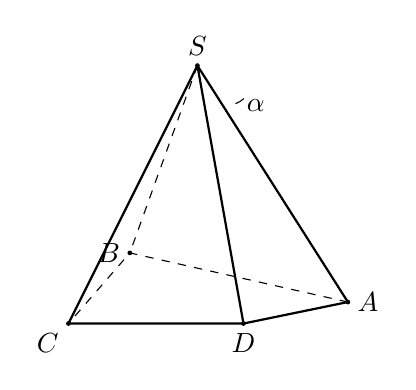
\begin{tikzpicture}[scale=0.78,>=stealth]
  \coordinate (S) at (2.1,4.2);
  \coordinate (B) at (1.0,1.15);
  \coordinate (A) at (4.55,0.35);
  \coordinate (D) at (2.85,0.0);
  \coordinate (C) at (0,0.0);
  \draw[thick] (S)--(C) (S)--(D) (S)--(A);
  \draw[dashed] (S)--(B);
  \draw[thick] (C)--(D)--(A);
  \draw[dashed] (A)--(B)--(C);
  \draw (2.72,3.58) arc (-70:-48:0.42);
  \node at (3.05,3.55) {$\alpha$};
  \fill (S) circle (1.1pt) node[above] {$S$};
  \fill (A) circle (1.1pt) node[right] {$A$};
  \fill (B) circle (1.1pt) node[left] {$B$};
  \fill (C) circle (1.1pt) node[below left] {$C$};
  \fill (D) circle (1.1pt) node[below] {$D$};
\end{tikzpicture}
\end{center}
\nopagebreak[4]
\Needspace{4\baselineskip}
\textbf{解析}

\Needspace{5\baselineskip}
取

\nopagebreak[4]
\[
B=(0,0,0),\quad A=(1,0,0),\quad
C=(0,1,0),\quad D=(1,1,0),\quad
S=(0,0,\sqrt3).
\]

\Needspace{5\baselineskip}
则

\nopagebreak[4]
\[
\overrightarrow{SA}=(1,0,-\sqrt3),\qquad
\overrightarrow{SD}=(1,1,-\sqrt3).
\]

\Needspace{5\baselineskip}
两向量的夹角为 $\alpha$，所以

\nopagebreak[4]
\[
\cos\alpha=\frac{4}{2\sqrt5}=\frac2{\sqrt5},
\qquad
\sin\alpha=\frac1{\sqrt5}.
\]

\gkanswer{答案：$\sin\alpha=\dfrac1{\sqrt5}$}

\end{answer}
\begin{answer}
\gksolhead{23}{}

\textbf{题目}：

\Needspace{5\baselineskip}
在双曲线

\nopagebreak[4]
\[
x^2-y^2=1
\]

的右支上求点 $P(a,b)$，使该点到直线 $y=x$ 的距离为 $\sqrt2$。

\Needspace{4\baselineskip}
\textbf{解析}

\Needspace{5\baselineskip}
在双曲线右支上，点 $P=(a,b)$ 满足 $a>0$ 且 $a^2-b^2=1$。到直线 $y=x$ 的距离为 $\sqrt2$，故

\nopagebreak[4]
\[
\frac{|b-a|}{\sqrt2}=\sqrt2,
\qquad |b-a|=2.
\]

\Needspace{5\baselineskip}
若 $b-a=2$，代入双曲线得 $a=-5/4$，不在右支；故 $b-a=-2$。于是

\nopagebreak[4]
\[
b=a-2,\qquad a^2-(a-2)^2=1,
\]

\Needspace{5\baselineskip}
从而

\nopagebreak[4]
\[
a=\frac54,\qquad b=-\frac34.
\]

\gkanswer{答案：$P=\left(\dfrac54,-\dfrac34\right)$}

\end{answer}
\begin{answer}
\gksolhead{24}{}

\textbf{题目}：

\Needspace{5\baselineskip}
解不等式：

\nopagebreak[4]
\[
\lg\left(x-\frac1x\right)<0.
\]

\Needspace{4\baselineskip}
\textbf{解析}

\Needspace{5\baselineskip}
先要求真数为正：

\nopagebreak[4]
\[
x-\frac1x>0,
\]

\Needspace{5\baselineskip}
得到 $x\in(-1,0)\cup(1,+\infty)$。又 $\lg(\cdot)<0$ 等价于

\nopagebreak[4]
\[
0<x-\frac1x<1.
\]

\Needspace{5\baselineskip}
在负区间和正区间分别解二次不等式，得到

\nopagebreak[4]
\[
x\in\left(-1,\frac{1-\sqrt5}{2}\right)
\cup
\left(1,\frac{1+\sqrt5}{2}\right).
\]

\gkanswer{答案：$\displaystyle\left(-1,\frac{1-\sqrt5}{2}\right)\cup\left(1,\frac{1+\sqrt5}{2}\right)$}

\end{answer}
\begin{answer}
\gksolhead{25}{}

\textbf{题目}：

\Needspace{5\baselineskip}
一个数列 $\{a_n\}$：当 $n$ 为奇数时，

\nopagebreak[4]
\[
a_n=5n+1;
\]

\Needspace{5\baselineskip}
当 $n$ 为偶数时，

\nopagebreak[4]
\[
a_n=2^{n/2}.
\]

求这个数列的前 $2m$ 项的和（$m$ 是正整数）。

\Needspace{4\baselineskip}
\textbf{解析}

\Needspace{5\baselineskip}
前 $2m$ 项中奇数项为

\nopagebreak[4]
\[
\sum_{k=1}^{m}\left[5(2k-1)+1\right]
=\sum_{k=1}^m(10k-4)
=5m^2+m.
\]

\Needspace{5\baselineskip}
偶数项和为

\nopagebreak[4]
\[
\sum_{k=1}^{m}2^k=2^{m+1}-2.
\]

\Needspace{5\baselineskip}
所以前 $2m$ 项和为

\nopagebreak[4]
\[
5m^2+m+2^{m+1}-2.
\]

\gkanswer{答案：$5m^2+m+2^{m+1}-2$}

\end{answer}